\newpage
\begin{center}
  \textbf{\large 2. Методы исследования}
\end{center}
\refstepcounter{chapter}
\addcontentsline{toc}{chapter}{2. Методы исследования}

Существуют различные подходы к моделированию кавитации, поэтому выбор модели и метода зависит от условий конкретной задачи.

Численные методы для моделирования кавитационных потоков можно разделить на два основных подхода: методы отслеживания границы раздела и методы континуальной модели.~\cite{10.1016/s1001-6058(11)60389-3}

Методы отслеживания границы предполагают наличие четкой границы между жидкостью и газом, которая определяется итеративным способом. Эти методы подходят для простых задач, где кавитационная область представляет собой хорошо определённый закрытый объем чистого газа.~\cite{10.1016/s0021-9991(03)00087-1, 10.1063/1.868709}

Континуальные методы рассматривают среду как двухфазную смесь с непрерывным изменением плотности между жидкостью и паром, не отслеживая границу раздела. Они широко применяются в задачах, связанных с турбулентными потоками, характерными для большинства промышленных процессов. Существуют три основные реализации континуальных методов: однофазные, двухфазные и гибридные.~\cite{10.1016/j.compfluid.2009.03.001}

Методы двухфазного моделирования предполагают, что жидкая и газовая фазы сосуществуют в каждой точке потока, и для каждой из них используется отдельная система уравнений сохранения. Таким образом, движение жидкости и пузырьков рассматривается раздельно, а две системы уравнений решаются совместно.~\cite{10.1017/s0022112000003098, 10.1143/jpsj.75.104401} Обычно изменение объема пузырьков описывается уравнением Релея-Плессе или его аналогами, а обмен массой, импульсом и энергией между фазами явно учитывается через специальные уравнения переноса. Это позволяет моделям учитывать физические особенности кавитации. Однако такие подходы сильно зависят от точности оценки взаимодействия между жидкостью и пузырьками, для которого не существует универсальной физической модели. Эти методы чаще всего применяются для потоков с умеренной кавитацией.~\cite{10.1002/fld.833, 10.1016/s1001-6058(08)60117-1}

В отличие от двухфазных, однофазные методы рассматривают среду кавитационного потока как однородную смесь, пренебрегая разницей скоростей между жидкостью и газом. Свойства смеси определяются на основе объемной доли газовой фазы, что делает среду псевдооднородной с резким изменением плотности от жидкой к газообразной фазе. Для расчета плотности смеси был предложен метод~\cite{delannoy1990two}, связывающий плотность с статическим давлением, который впоследствии был улучшен~\cite{10.1115/1.1596239} с использованием уравнения состояния для локально однородной сжимаемой двухфазной среды в условиях равновесия. Далее, была предложена модель~\cite{10.1017/s002211209200003x} двухфазной кавитации с использованием уравнения Релея-Плессе для описания динамики пузырьков, и разработана полную модель кавитации ~\cite{10.1115/1.1486223}, учитывающая перенос массы через эмпирически определяемый источник для транспорта газовой фракции. Хотя однофазные методы не могут описать сильные термодинамические или кинетические неравновесия, они проще в реализации и вычислительно менее затратны, поскольку не требуют раздельного учета движения пузырьков.  

Гибридные методы занимают промежуточное положение между однофазными и двухфазными подходами. Они создаются путем добавления уравнений массы для плотности газа или жидкости с учетом источника кавитации в рамках однофазных моделей.~\cite{10.1016/s0045-7930(99)00039-0, 10.1007/s00773-003-0162-6} Основная сложность таких методов заключается в формулировке источника кавитации и настройке параметров, связанных с процессами испарения и конденсации.

Турбулентность также является важным аспектом моделирования кавитации. Для учёта её влияния часто применяются методы, такие как осреднённые по Рейнольдсу уравнения Навье-Стокса (RANS). Однако стандартные модели турбулентности имеют ограничения, например, чрезмерное производство вихревой вязкости, что затрудняет моделирование нестационарных процессов, таких как колебания кавитационных пузырьков.  

Численные схемы для расчета кавитационных потоков сталкиваются с дополнительными трудностями из-за больших локальных изменений числа Маха. Для корректного описания практически несжимаемых жидкостей и высоко сжимаемых кавитационных областей требуются модификации алгоритмов давления, например, SIMPLE или PISO.~\cite{10.1006/jcph.2002.6992, 10.1016/s0045-7930(98)00061-9} Однако такие модификации могут приводить к ошибкам в оценке скорости звука, особенно на границе фаз. Для преодоления этой проблемы разработаны предобусловленные методы, позволяющие улучшить сходимость расчетов.  

Современные подходы, такие как улучшенные алгоритмы CIP-CUP, демонстрируют эффективность в условиях резкого изменения скорости звука в кавитационных областях. Эти методы направлены на повышение точности и надежности моделирования в промышленных и научных задачах.~\cite{10.1016/s1001-6058(11)60389-3}


\section{Метод конечных объёмов}
В нашем исследовании мы анализируем поведение последовательности лазерно-индуцированных кавитационных пузырей вблизи торца волокна с помощью компьютерного моделирования методом конечных объёмов (МКО). 
Метод конечных объёмов (МКО) — это численный подход, основанный на дискретизации интегральных законов сохранения (массы, импульса, энергии) для отдельных ячеек расчетной области. 
В отличие от методов, работающих с дифференциальными уравнениями, МКО учитывает баланс потоков физических величин через границы каждой ячейки, что обеспечивает строгое выполнение законов сохранения даже на грубых сетках. 
Ключевая особенность метода — интегро-интерполяционный подход: исходные уравнения интегрируются по объёму ячейки, а потоки через её границы аппроксимируются с выбранным порядком точности. 
Это делает МКО особенно эффективным для задач с разрывными решениями (ударные волны, фазовые переходы) и сложными геометриями, так как он естественным образом сохраняет физическую согласованность решения. 
Благодаря этим свойствам метод широко применяется в вычислительной гидродинамике, теплообмене и моделировании многофазных течений, включая кавитационные процессы.
МКО хорошо подходит для моделирования кавитации, поскольку позволяет точно описывать резкие изменения плотности и давления в зонах перехода между жидкостью и газом. 
Кроме того, метод хорошо адаптируется к сложным геометриям и может учитывать нестационарные явления, такие как схлопывание пузырьков, что делает его универсальным инструментом для анализа сложных двухфазных потоков.


Наша работа включает детальное исследование ударной волны, возникающей при коллапсе пузырей, и распределения таких параметров, как давление, температура и скорости.
Эти параметры важны для оценки воздействия на окружающие материалы и структуры.
Полученные результаты способствуют более глубокому пониманию явления кавитации и могут привести к повышению безопасности, точности и эффективности различных технологий, основанных на кавитации.

В основе нашего моделирования используется уравнение Навье-Стокса, которое описывает движение вязкой жидкости, дополненное уравнениями неразрывности для обеспечения сохранения массы и импульса в системе:
\begin{equation*}
    \frac{\partial (\rho \mathbf{U})}{\partial t} + \nabla \cdot (\rho \mathbf{U} \otimes \mathbf{U}) = -\nabla p + \nabla \cdot \mathbf{T}
    + \int_{S(t)} \sigma \kappa (\mathbf{x'}) \hat{n}(\mathbf{x'}) \delta (\mathbf{x} - \mathbf{x'}) \, dS' ,
\end{equation*}

\begin{equation*}
    \frac{\partial \rho}{\partial t} + \nabla \cdot (\rho \mathbf{U}) = 0
\end{equation*}

\begin{equation*}
    \frac{\partial (\alpha_i \rho_i)}{\partial t} + \nabla \cdot (\alpha_i \rho_i \mathbf{U}) = 0
\end{equation*}

, где
\begin{equation*}
    \mathbf{T} = \mu \left( \nabla \mathbf{U} + (\nabla \mathbf{U})^T - \frac{2}{3} (\nabla \cdot \mathbf{U}) \mathbf{I} \right)
\end{equation*}

– тензор вязких напряжений ньютоновской жидкости, $\mathbf{I}$ – единичный тензор, поверхностное натяжение $\sigma$ считается постоянным, поверхностный интеграл представляет собой поверхностную силу, действующую на границе раздела жидкость/газ,  $\kappa$ – удвоенная средняя кривизна границы раздела, $\hat{n}$ – единичная нормаль к поверхности.

Для расчета изменения давления и плотности во времени использовались уравнения состояния, такие как уравнение Тейта для жидкости:
\begin{equation*}
    \rho = \rho_0 \bigg(\frac{p + B}{p_0 + B}\bigg)^{\frac{1}{\gamma}}
\end{equation*}

и уравнение состояния идеального газа для пара:
\begin{equation*}
    \rho = \frac{p}{R T}
\end{equation*}

Такой подход обеспечил точное воспроизведение поведения кавитационного пузыря, включая распределение параметров, таких как давление, температура и поля скоростей, что необходимо для оценки их влияния на прилегающие материалы и структуры~\cite{10.1016/j.compfluid.2015.11.008}.

Моделирование проводилось при помощи open-source пакета для моделирования методом конечных объемов OpenFOAM.
В качестве метода решения использовался метод compressibleInterFoam, предназначенный для моделирования переходных процессов двух сжимаемых, неизотермических и несмешивающихся жидкостей.
Он обрабатывает ламинарные и турбулентные потоки жидкости и использует метод определения объема жидкости (VoF) для точного определения границы раздела.
Метод compressibleInterFoam основан на алгоритме PIMPLE -- это алгоритм для связи давления и импульса, сочетающий преимущества алгоритмов PISO (Pressure-Implicit with Splitting of Operators) и SIMPLE (Semi-Implicit Method for Pressure-Linked Equations). 
Он широко применяется в CFD-расчётах для решения несжимаемых и слабосжимаемых течений, особенно в задачах с большими временными шагами (критерий Куранта > 1), сложной геометрией, нестационарными процессами.
Алгоритм итеративно решает систему уравнений Навье-Стокса, связывая давление и скорость через поправки.
Работа алгоритма состоит из следющих шагов: предиктор скорости, коррекция давления, коррекция скорости и при необходимости итеративная стабилизация.
Этот алгоритм является гибким решением, сочетающим быстроту PISO (для малых шагов) и устойчивость SIMPLE (для больших шагов), с возможностью опциональной итеративной стабилизации.

\section{Определение фаз}
В нашей модели учитывались разные фазы -– жидкость и газ -- для определения фаз используется метод Volume of Fluid (VoF) -- это численный подход для моделирования многофазных течений, в котором положение границы раздела фаз (например, жидкость-газ) определяется с помощью доли объема (volume fraction) $\alpha$ каждой фазы в расчетных ячейках.
В ходе работы метода изначально каждой ячейке этот параметр задается исходя из начальных условий: $\alpha$ = 0 — ячейка полностью заполнена газом, $\alpha$ = 1 — ячейка полностью заполнена жидкостью, 0 < $\alpha$ < 1 — ячейка содержит межфазную границу.
Далее на каждом временном шаге для каждой ячейки решается дифференциальное уравнение переноса, описывающее, в том числе, эволюцию межфазной границы, и на основе полученного решения и предыдущих значений с помощью аппроксимации для поддержания неразрывности восстанавливается граница раздела.
Такой подход позволяет отслеживать эволюцию фаз и точно моделировать формирование кавитационных пузырей и их взаимодействие с окружающей средой.
Для разделения двух фаз вводятся объемные доли жидкости $\alpha _ {l} = \alpha$ и газа $\alpha _ {g}$:
\begin{equation*}
    \alpha _ {g}  (x,t) = 1 - \alpha _ {l}  (x,t)
\end{equation*}

Полные плотность и вязкость можно записать в виде:
\begin{gather*}
    \rho  (x,t)=  \alpha _ {l}  (x,t)  \rho _ {l}  (x,t)+  \alpha _ {g}  (x,t)  \rho _ {g}  (x,t) \\
    \mu  (x,t)=  \alpha _ {1}  (x,t)  \mu _ {1}  +  \alpha _ {g}  (x,t)  \mu _ {g}
\end{gather*}

\section{Параметры моделирования}
Расчетная область моделирования представляет собой вытянутый эллипсоид с двумя полуосями, равными $1.2 \cdot 10^{-2}$ м, и третьей полуосью, равной $1.6 \cdot 10^{-2}$ м.
На одном из торцов эллипсоид имеет вырезанную часть в форме цилиндра для имитации образца ткани высотой $0.6 \cdot 10^{-2}$ м и радиусом основания $r_t = 1.5 \cdot 10^{-4}\text{ м}$.
В качестве жидкости используется вода при нормальных условиях (давление $p=10^5$ Па).
На конце ткани задается полость радиусом $r_c = 1.5 \cdot 10^{-4}\text{ м}$, наполненная газом с повышенным относительно воды давлением $p_1$ (рис.~\ref{fig:initial_parameters}).
Моделирование состояло из нескольких серий с одиночным и тройным импульсом.
В случае тройного импульса 1й импульс появляется в при запуске моделирования, 2й и 3й импульсы создают полости того же размера с давлением $p_2$ и $p_3$ соответственно, 2й импульс инициируется через $3.5\cdot10^{-5}$ c после запуска моделирования, 3й -- через $7\cdot10^{-5}$ c.
Значение $p_1$ варьируется в диапазоне $\approx 10^6\text{ Па} - 10^8\text{ Па}$.
Значения давлений в следующих полостях также варьируются $p_2 \approx 0.25 p_1 - 4p_1$, $p_3 \approx 0.25 p_1 - 4p_1$.

\begin{figure}[h!]
    \centering
    % First row
    \begin{subfigure}{.45\textwidth}
        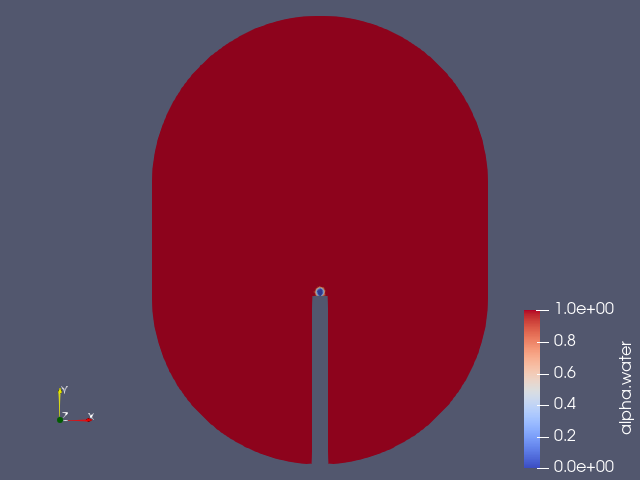
\includegraphics[width=\textwidth]{images/alphawater_0.png}
        \centering \caption{}
    \end{subfigure}
    \hspace{1cm}
    \begin{subfigure}{.45\textwidth}
        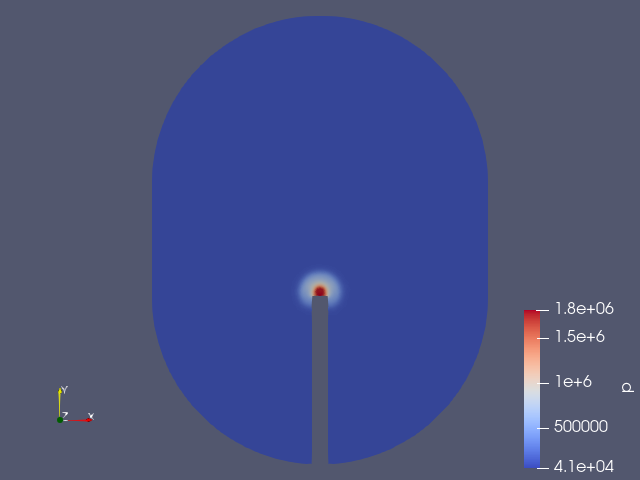
\includegraphics[width=\textwidth]{images/pressure_0.png}
        \centering \caption{}
    \end{subfigure}
    
    \caption{Распределение фаз (а) и давления (б) в начальный момент времени моделирования}
    \label{fig:initial_parameters}
\end{figure}

На стенках цилиндра заданы граничные условия типа zeroGradient, что соответствует условию равенства нулю нормального градиента физических величин и является моделью непроницаемой жесткой стенки. 
На внешней границе расчетной области (стенках ограничивающего эллипсоида) применены waveTransmissive граничные условия, специально разработанные для нерефлектирующего пропускания акустических и ударных волн из расчетной области, что минимизирует отражения и обеспечивает корректное моделирование волновых процессов в открытой системе.

Для построения сетки использовался пакет SALOME, позволяющий сгенерировать пространственную сетку для выбранной геометрии при помощи гибридного алгоритма, который сначала выполняет разбиение заданных фигур и поверхностей на простые топологические элементы (тетраэдры, гексаэдры, призмы), а затем оптимизирует сетку с учетом заданных критериев качества, таких как минимальный угол, ортогональность, плавность изменения размеров ячеек.
Отличительной особенностью данного решения является поддержка адаптивных методов, позволяющих легко контролировать точность сетки в выбранных областях, что являлось необходимым для моделирования кавитационного процесса, так как ввиду нелинейных процессов вблизи появившейся полости необходима высокая точность решения в этой зоне для получения корректной границы фаз и распределения параметров на этой границе.
В результате была получена сетка, удовлетворяющая данным требованиям (рис.~\ref{fig:mesh})

\begin{figure}[h!]
    \centering
    % First row
    \begin{subfigure}{.45\textwidth}
        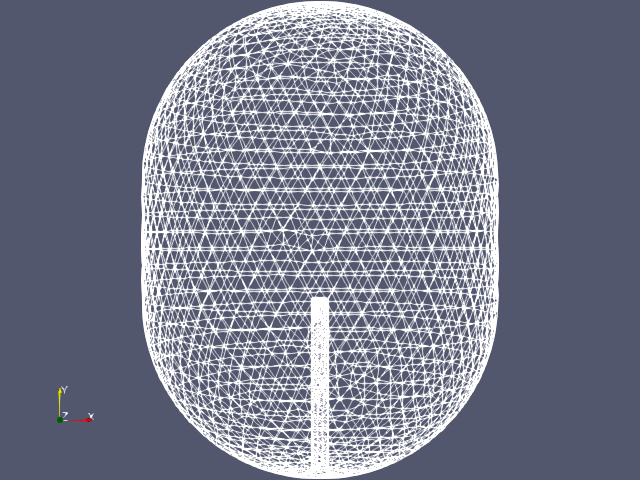
\includegraphics[width=\textwidth]{images/mesh_3d.png}
        \centering \caption{}
    \end{subfigure}
    \hspace{1cm}
    \begin{subfigure}{.45\textwidth}
        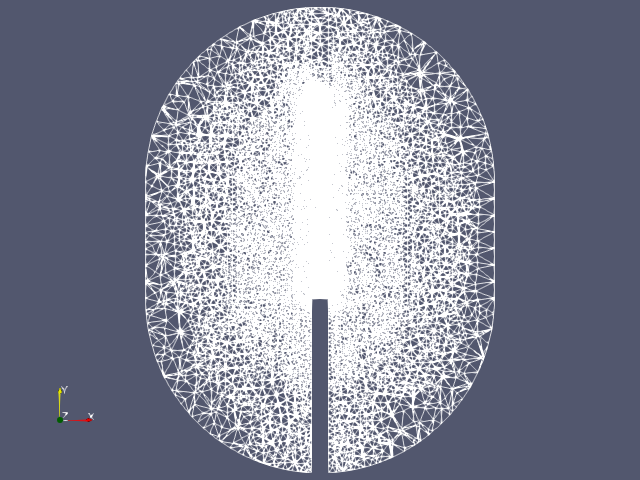
\includegraphics[width=\textwidth]{images/mesh_2d.png}
        \centering \caption{}
    \end{subfigure}
    
    \caption{(а) Пространственная сетка границы области моделирования, (б) сетка моделирования в разрезе}
    \label{fig:mesh}
\end{figure}


В ходе численного моделирования используется алгоритм адаптивного выбора временного шага интегрирования (см. Приложение А), что обусловлено наличием существенных нелинейностей в решаемой системе уравнений, вызванных резкими градиентами гидродинамических параметров, которые делают неприменимыми методы с фиксированным временным шагом ввиду их расходимости при данных условиях.
Длительность моделирования составляет $2\cdot10^{-3}$ c, всего выходит $\approx$ 400 кадров моделирования.

\section{Пост-обработка эксперимента}
Для обработки и выделения фаз из черно-белого изображения эксперимента использовался алгоритм, состоящий из предобработки и постобработки изображения и анализа площади.

На этапе предобработки выполнялись следующие шаги:
\begin{itemize}
    \item обрезка изображений к одному размеру
    \item гауссово размытие (3×3): уменьшает высокочастотный шум, сохраняя границы пузырей
    \item адаптивная бинаризация: локально разделяет фон и объекты с учетом неравномерного освещения
    \item CLAHE (Contrast Limited Adaptive Histogram Equalization): улучшает контраст в теневых областях без пересвета
\end{itemize}

На этапе постобработки выполнялись следующие шаги:
\begin{itemize}
    \item маскирование области интереса: исключает область ткани из анализа
    \item адаптивная бинаризация: оптимизирована для выделения границ пузырей.
\end{itemize}

После проведения предобработки и постобработки получаем бинарное изображение по фазам (рис.~\ref{fig:postprocess}), на основе которого проводится анализ площади, то есть подсчет пикселей нужной фазы. 

\begin{figure}[h!]
    \centering
    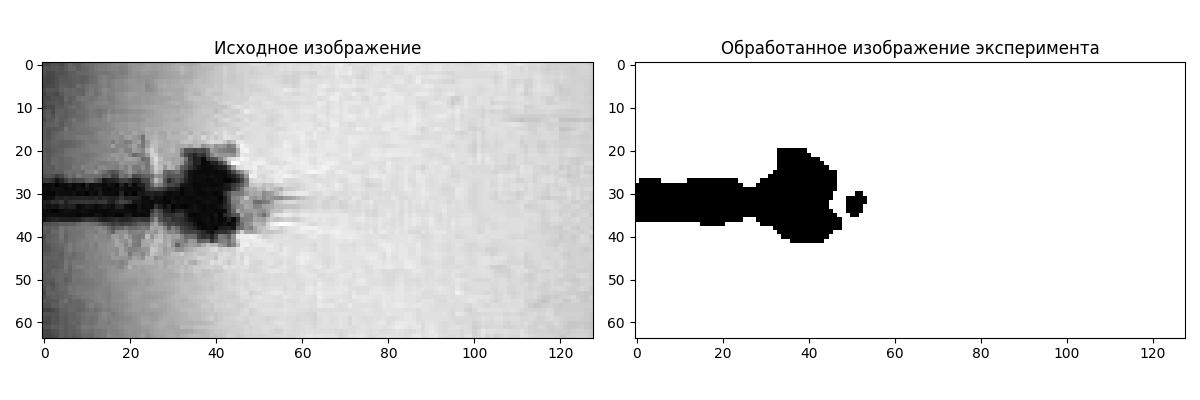
\includegraphics[width=0.95\linewidth]{images/postprocess.jpg}
    \caption{Пример результата постобработки изображения эксперимента}
    \label{fig:postprocess}
\end{figure}